%!TEX root = ../thesis.tex

\section{Results}
In \autoref{fig:4_losses} we can see the evolution of training and validation
loss during a 200 epochs run. In this run, the NN as described in chapter 3 and
the training data as described in chapter 2 was used. The NN converges fast
until about epoch 60. After epoch 60 training and validation loss start to
slowly diverge, indicating that the NN started to overfit on the training data.
Apparently it even converges a little bit faster than the corresponding 
experiment in \cite{PhysRevD.105.043002}.
\footnote{According to Ondřej Zelenka in a private discssion on Slack on
  24.01.22} I accord this to the difference in training set. The state of the
NN at epoch 59 was chosen as the \hlc{best\_weights.pt}.

\begin{figure}[ht]
  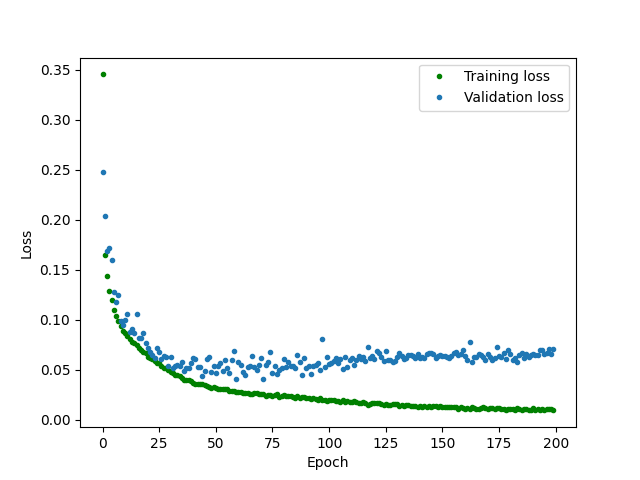
\includegraphics[width=\textwidth]{img/4_results/losses.png}
  \caption{Training and validation loss over 200 epochs.}
  \label{fig:4_losses}
  \centering
\end{figure}

In \autoref{fig:4_eff} we can see how the efficiency evolved over the 200 epochs.
Again we have a fast improvement of the efficiency and after about epoch 40 it
converged to about 0.9, which is similar to what the authors of
\cite{PhysRevD.105.043002} observed.

\begin{figure}[ht]
  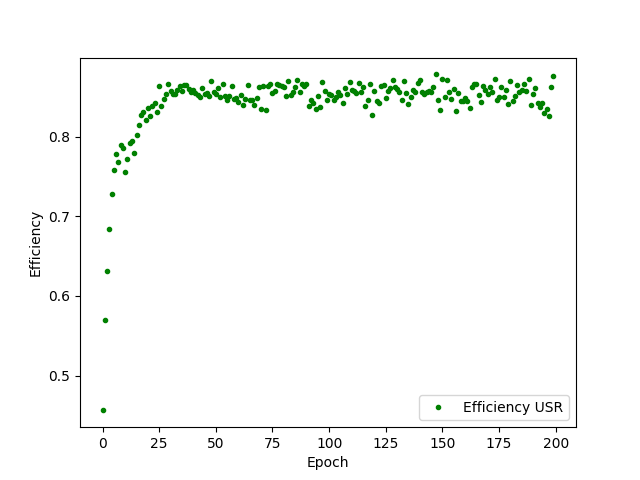
\includegraphics[width=\textwidth]{img/4_results/efficiencies.png}
  \caption{eff.}
  \label{fig:4_eff}
  \centering
\end{figure}

The low loss as well as the high efficiency are good indicators for a good
performance of our NN. To evaluate how good the NN actually is, two numerical
experiments were made. The first one was applying the network to a small test
set with short duration. The second one was applying the neural network to test
data of 1 month and computing a sensitivity plot.

\subsection{Experiment 1: Short Test Data}
In this experiment, a short strain of noise was generated and injected with 5
signals at different SNR. The whole strain was whitened and analyzed by the
neural network.

In \autoref{fig:4_apply_single} we can see a plot consisting of three windows.
The top window displays pure noise in blue with the 5 signals overlayed. Note
that it does in the top window, the signals are not yet injected into the noise.
In the middle window, we can see the whitened noise+signal strain. In the bottom
window, the p-score of the network is plotted.

As we can see, the network detects all signals and assigns a pscore of 1 for all
of them but it sometimes also assigns a high pscore value to noise. Noteworthy
is also the difference between the thickness of the bars in the bottom window.
The bars indicating signals are thicker because we use a sliding window to feed
the data to our NN, leading to several windows containing the same merger.

The result to this experiment made me confident, that the NN does indeed
recognize GW signals injected in whitened Gaussian noise.

\begin{figure}[ht]
  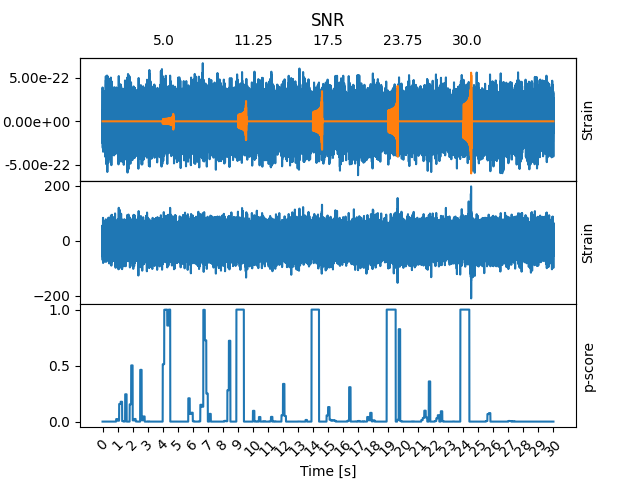
\includegraphics[width=\textwidth]{img/4_results/apply_single.png}
  \caption{apply single.}
  \label{fig:4_apply_single}
  \centering
\end{figure}

\subsection{Experiment 2: 1 Month of Test Data}
In this experiment, we analyze a month of test data, compute the FAR as well as
the sensitive distance and plot it. Computing the FAR as well as the
sensitivity distance is done with code prodived by \cite{MLGWSC1}.

\begin{figure}[ht]
  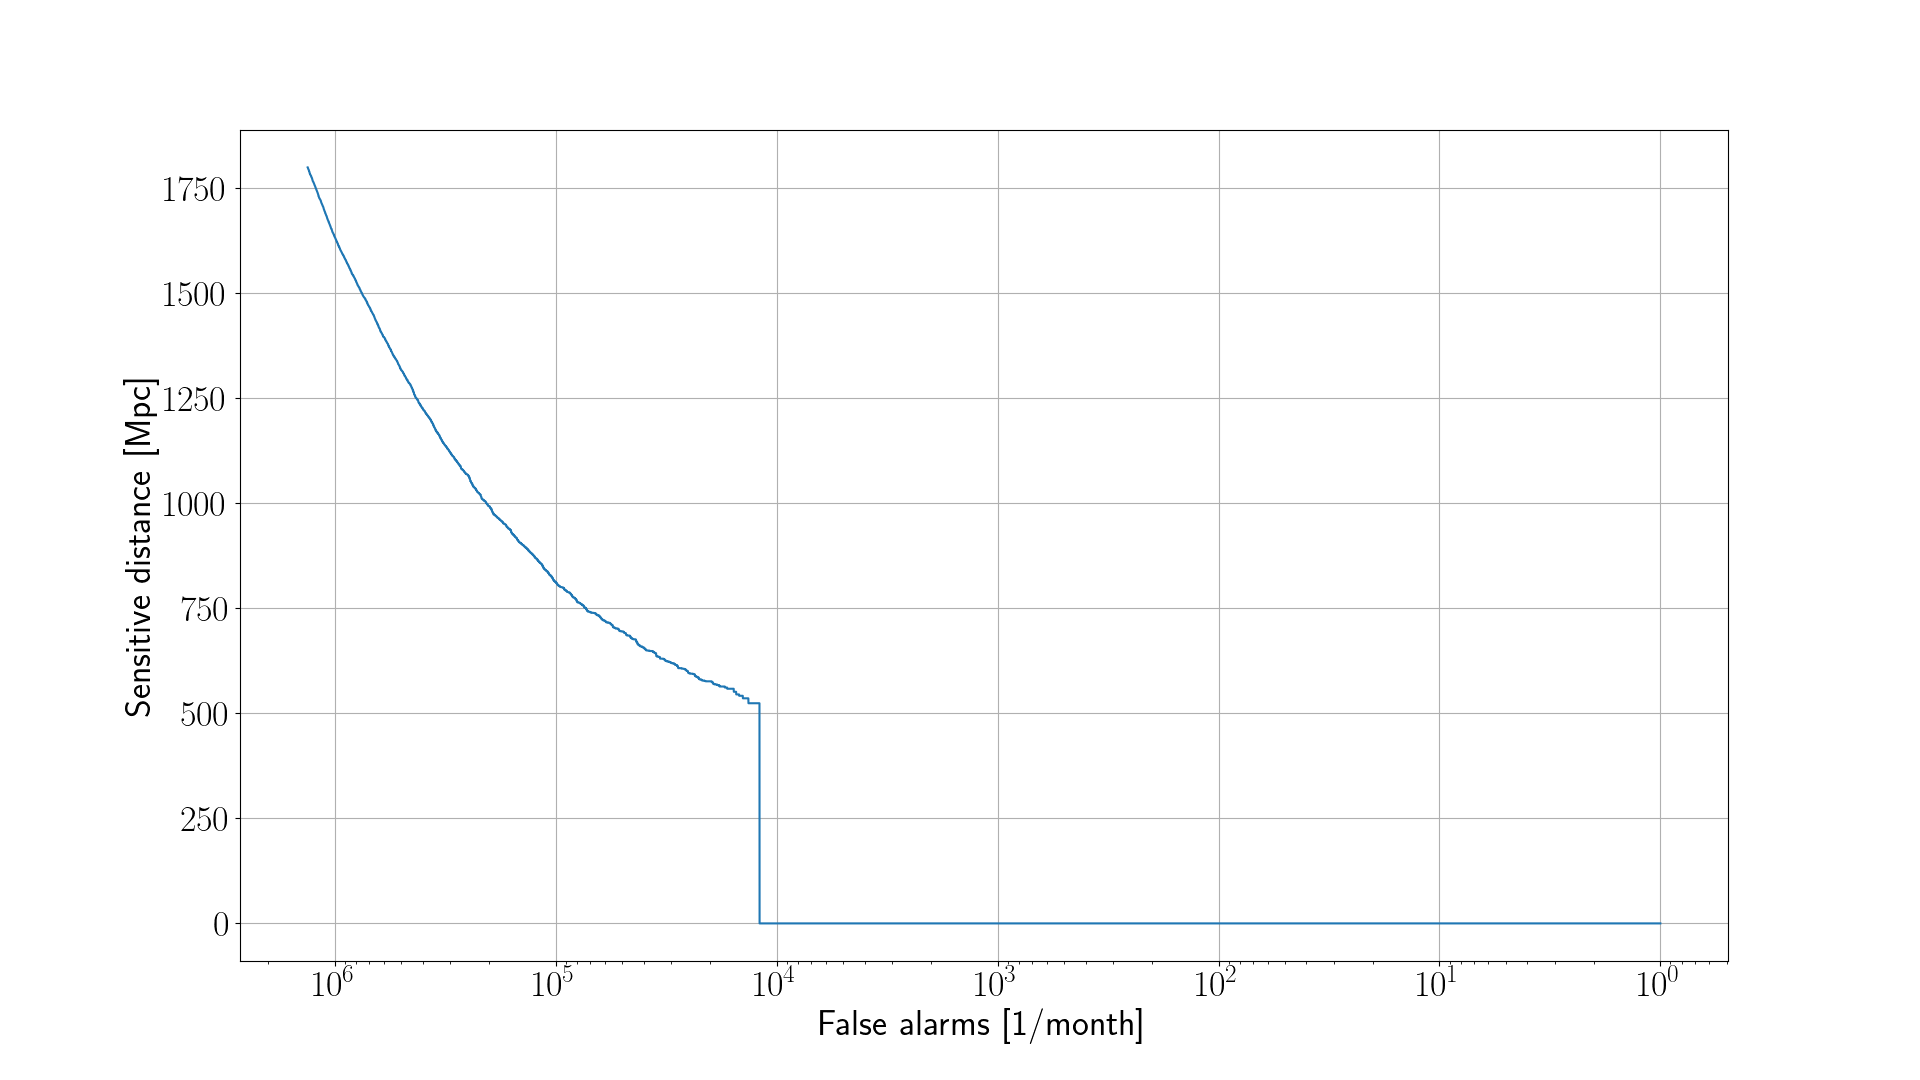
\includegraphics[width=\textwidth]{img/4_results/sensitivity_plot.png}
  \caption{The NN applied to short test data.}
  \label{fig:4_sensitivity_plot}
  \centering
\end{figure}

The plot indicates how many false alarms per month are found. For mergers which
are further away and thus are generally harder to measure we can expect a higher
number of false alarms. In the plot we can see this behaviour. Furthermore note
the sudden drop in sensitivity distance around $10^4$ false alarms. This is
because for this plot, the softmax output layer was used. If the USR output
layer would have been used, we would see a smooth continuation of the graph. The
reason this isn't included is because the corresponding data got lost in an
technical accident and reapplying the network would have taken too long on my
limited hardware.

While this plot seems to indicate a successfull analysis of test data, I think
it actually shows the opposite. In \hlc{MLGWSC/mock/ds1.ini} we can see that
we used a maximal
chirp distance of $350$ mpc. Because of this, I'd expect the maximal
sensitivity distance to be of around 6'000 and not 1750.

Despite this result, I'm still confident that the network itself works. This is
because of the first experiment. I think the issue that led to this bad result
can be found in the data pipeline used to split up the 1 month of data but in
the end, that's just a guess.

My conclusion is nevertheless positive. I was able to find GW signals injected
in Gaussian noise and got to explore the space of GW analysis using ML methods
in depth which presented itself as a challenging but instructive experience.

This thesis is hosted on
\url{https://github.com/pascal-mueller/bachelor_thesis}
